\documentclass{beamer}
\usepackage[utf8]{inputenc}
\usepackage[T1]{fontenc}
\usepackage[french]{babel}
\usepackage{colortbl}
\usepackage{verbatim}
\usepackage{amsmath}
  
\usetheme{Warsaw}

\title[Classification de documents]{Extraction de connaissances avancée\\ \emph{``Analyse d'opinion''}}
\author{Carbonnel Jessie \and Nguyen Daniel \and Pibre Lionel}
\institute[UM2]{Université de Montpellier 2}
\date{18 Décembre 2014}
\logo{
\includegraphics[height=10mm]{imgs/um2.png}}

\AtBeginSection[]
{
  \begin{frame}
  \frametitle{Sommaire}
  \tableofcontents[currentsection, hideothersubsections, hideothersections]
  \end{frame} 
}

\addtobeamertemplate{footline}{\insertframenumber/\inserttotalframenumber}

\setbeamertemplate{navigation symbols}{% 
}

\begin{document}

\begin{frame}
\titlepage
\end{frame}

\begin{frame}{Sommaire}
	\tableofcontents[hidesubsections]
\end{frame}
%%%%%%%%%%%%%%%%%
% SECTION
%%%%%%%%%%%%%%%%%
\section{Introduction}
\begin{frame}
	\begin{block}{Introduction}
		\textbf{Sujet:} Classification des opinions sur les commentaires des applications de Google Play Store.		
		
		\vspace{0.5cm}
		
		\textbf{Problématique:} Prédire la note que l'utilisateur va donner à une application à partir de son commentaire.
			
	\end{block}
\end{frame}

\section{Constitution du corpus}
\begin{frame}
	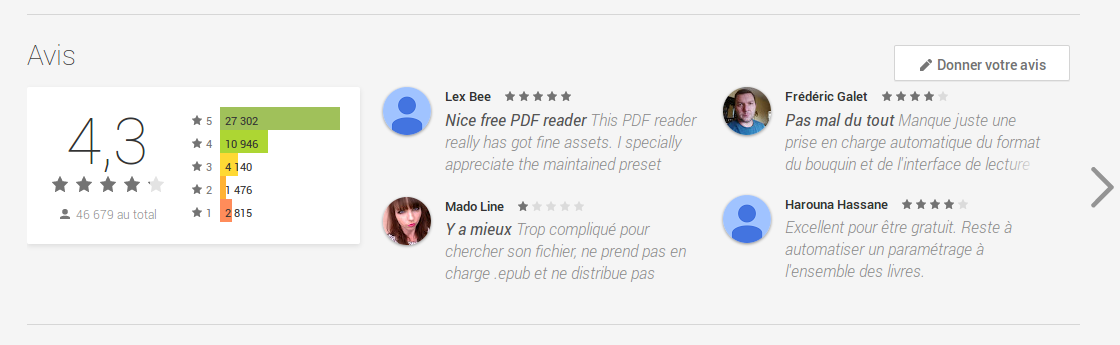
\includegraphics[width=\textwidth]{imgs/ebook.png}
\end{frame}


\begin{frame}
	\begin{block}{Structure des données récupérées}
%		\begin{verbatim}
			NomApplication:Ebook et PDF Reader

			IdApplication:books.ebook.pdf.reader

			CategorieApplication:Livres et références

			NoteApplication:4,3

			NombreVotants:43 379

			TitreCommentaire:Ebook Pelerin

			Commentaire: Super installation, ai acheté un ebook chez Bayard. Suis pas déçu.

			DateCommentaire:26 juillet 2014

			NoteCommentaire:5
%		\end{verbatim}
	\end{block}
\end{frame}

\section{Prétraitement et génération des fichiers ARFF}
\subsection{Prétraitement}
\begin{frame}
	\begin{block}{TreeTagger}
		Utilisation de TreeTagger afin d'avoir la classe grammaticale des mots ainsi que leur forme lemmatisée.
	\end{block}
	
\end{frame}

\begin{frame}
\begin{exampleblock}{Structure de sortie de TreeTagger}
			\centering
			 \begin{tabular}{|c|c|c|}
					\hline
					Mot&Classe grammaticale&Mot lemmatisé\\
					\hline
					dès&PRP&dès\\
					que&KON&que\\
					je&PRO:PER&je\\
					lance&VER:pres&lancer\\
					l'&DET:ART&le\\
					application&NOM&application\\
					j'&PRO:PER&je\\
					adore&VER:pres&adorer\\
					cyprien&ADJ&cyprien\\
					\dots&\dots&\dots\\
					\hline
			 \end{tabular}
	\end{exampleblock}

\end{frame}

\subsection{Génération des fichiers ARFF}
\begin{frame}
	\begin{block}{Génération}
		Programmation d'un parser en java.\\
		
		\textbf{Quatre fichiers de sortie:}
		\begin{itemize}
			\item Texte Brut
			\item Texte Brut Lemmatisé
			\item Texte Nettoyé
			\item Texte Nettoyé Lemmatisé
			\item Les quatre mêmes fichiers mais en corrigeant les mots adorer, aimer et kiffer
		\end{itemize}
	\end{block}
\end{frame}

\section{Visualisation}
\subsection{Camembert}
\begin{frame}
	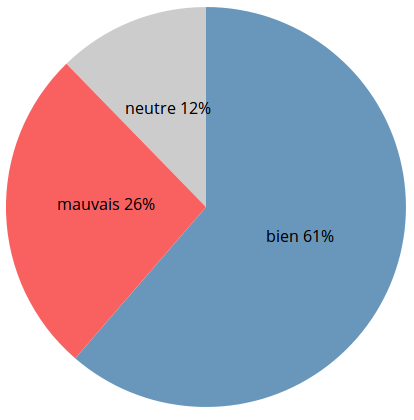
\includegraphics[height=5cm]{imgs/visu1.png}
\end{frame}

\subsection{Histogramme}
\begin{frame}
	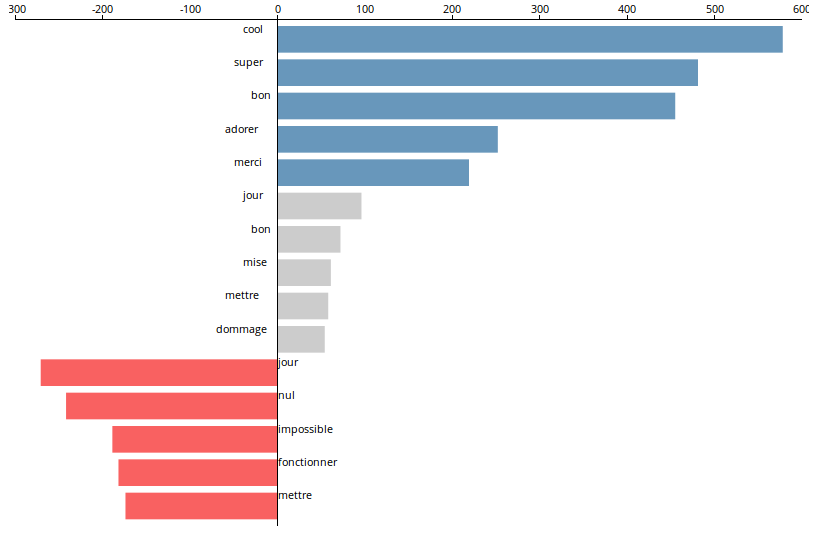
\includegraphics[height=5cm]{imgs/visu2.png}
\end{frame}

\section{Classification}

\begin{frame}
	\begin{block}{Algorithmes utilisés}
		\begin{itemize}
			\item NaiveBayes: probabiliste (théorème de Bayes)
			\item J48: arbre de décision
			\item JRip: règles d'association
			\item SMO: machine à vecteurs de support
			\item IBk: K plus proches voisins
		\end{itemize}
	\end{block}
\end{frame}

\begin{frame}
	\begin{block}{Méthodes utilisées}
		\begin{itemize}
			\item Utilisation de la représentation \textbf{sac de mots}
			\item Première exécution avec la présence des mots (représentation binaire)
			\item Deuxième exécution avec l'occurence des mots (représentation fréquentiste)
		\end{itemize}
	\end{block}
\end{frame}

\begin{frame}
	\begin{block}{Les problèmes liés au corpus}
		\begin{itemize}
			\item Certains commentaires sont écrits en anglais
			\item Fautes d'orthographe et de frappe
		\end{itemize}
		
		\vspace{0.5cm}
		
		$\Rightarrow$ \textbf{Les mots avec des fautes ou en anglais ne sont pas reconnus par TreeTagger}
	\end{block}
\end{frame}

\begin{frame}
	\begin{exampleblock}{Fautes d'orthographe et de frappe}
		``Je kiff grave car jadore cyprien et jaimefai lui poser un question : est ce que tu connais squeezie ( ca c oui c sur ) norman kihouu tal blackm ....''\\
		
	\end{exampleblock}
	
	\begin{exampleblock}{Commentaire en anglais}
		``It keeps loosing my books , I have to re-download them every day''
	\end{exampleblock}

\end{frame}

\begin{frame}
	\begin{block}{Résultats des instances correctments classifiées}
	\begin{minipage}{0.4\textwidth}\center
		\textbf{Texte Brut}
		\begin{description}
			\item[SMO: ]73,1\%
			\item[J48: ]67,8\%
			\item[IBk: ]65,6\%
			\item[JRip: ]64,8\%
			\item[NaiveBayes: ]64,2\%
		\end{description}	
		\end{minipage}
		\begin{minipage}{0.4\textwidth}\center
		\textbf{Texte Brut Lemmatisé}
		\begin{description}
			\item[SMO: ]73,6\%
			\item[J48: ]68,9\%
			\item[IBk: ]65,9\%
			\item[JRip: ]67,8\%
			\item[NaiveBayes: ]65,9\%
		\end{description}	
		\end{minipage}
	\end{block}
\end{frame}

\begin{frame}
	\begin{block}{Analyses des résultats}
	\begin{itemize}
		\item L'algorithme SMO est le plus robuste.
		\item Text brut $\Rightarrow$ Les mêmes mots sont écrits différemment
		\item Texte brut lemmatisé $\Rightarrow$ Les mots non reconnus disparaissent
		\item Texte lemmatisé $\Rightarrow$ Certains commentaires peuvent être vides
	\end{itemize}

	\end{block}
\end{frame}

\begin{frame}
	\begin{block}{Résultats des instances correctments classifiées sur le texte corrigé}
		\begin{description}
			\item[SMO: ]73,2\%
			\item[J48: ]67,8\%
			\item[IBk: ]65,6\%
			\item[JRip: ]65,2\%
			\item[NaiveBayes: ]64,3\%
		\end{description}	
		
		Texte corrigé $\Rightarrow$ Meilleurs résultats
	\end{block}
\end{frame}

\section{Conclusion et perspectives}
\begin{frame}
	\begin{block}{Conclusion}
		\begin{itemize}
			\item Suivre un processus de fouille de données de A à Z
			\item Voir les différents résultats suivant le corpus
			\item L'impact des fautes d'orthographe sur les résultats
		\end{itemize}
	\end{block}
\end{frame}

\begin{frame}
	\begin{block}{Perspectives}
	
	\begin{itemize}
		\item Utiliser des outils de TALN pour corriger le corpus et traduire les commentaires écrits en anglais
		\item Faire de nouvelles visualisations sur les résultats obtenus
		\item Tester d'autres algorithmes
	\end{itemize}
	
	\end{block}
\end{frame}

\end{document}
